\chapter{Projekt architektury systemu}
\label{cha:projektSystemu}
W tym rozdziale omówiona zostanie architektura implementowanego systemu. W pierwszym podrozdziale znajduje się ogólny opis używanej archikterktury, w następnym model bazy danych, który poprzedza model klas. W czwartym podrozdziale przedstawiony jest diagram sekwencji.
\section{Opis architektutry}
Implementowany projekt jest oparty na architekturze SOA (wyjaśnionej w podrozdziale \ref{sec:soa}), która została wybrana przede wszystkim ze względu na podział aplikacji na niezależne od siebie moduły. Dzięki modularności w łatwy sposób można dodawać nowe funkcjonalności do projektu poprzez wstawianie kolejnych usług. Oprócz opisanej wcześniej architektury do implementacji projektu został użyty wzorzec projektowy MVC (\textit{ang. Model View Controller}), który jak sama nazwa wskazuje odpowiada za podzielenie aplikacji na trzy częśći:
\begin{itemize}
	\item Model - część odpowiedzialna za zarządzanie danymi czyli za połączenie z bazą danych,
	\item View - widok odpowiada za interakcję użytkownika z systemem czyli graficzny interfejs użytkownika,
	\item Controller - kontroler oddziałuje pomiędzy modelem a widokiem i kontroluje przepływ danych pomiędzy nimi. \cite{MVC01}
\end{itemize}
MVC jest na niższym poziomie abstrakcji niż SOA dzięki czemu mogą razem koegzystować. 

Opisywaną architekturę przedstawia poniższy model komponentów:
\begin{figure}[H]
\centering
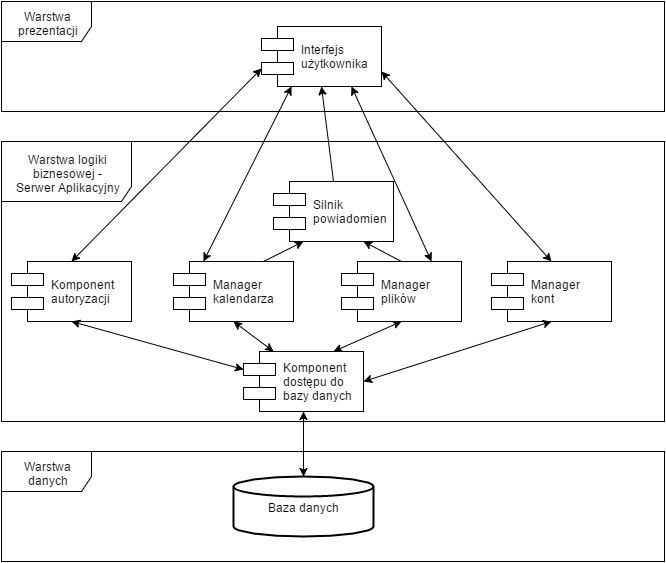
\includegraphics[scale=0.5]{ArchitekturaSystemu}
\caption{\label{fig:diag_01}Diagram komponentów}
\end{figure}
Gdzie każdy z komponentów zostanie opisany dokładnie w rozdziale implementacyjnym.

\section{Model bazy danych}
\label{sec:bd}
Baza danych składa się z sześciu tabel:
\begin{itemize}
	\item User - odpowiedzialna za przechowywanie danych o użytkownikach,
	\item Role - Wyznaczająca rolę użytkownika: \textit{user} lub \textit{admin}, dzięki którym można rozróżnić uprawnienia,
	\item File - Reprezentuje plik,
	\item Calendar - odpowiedzialny za przechowywanie kalendarza użytkownika,
	\item Event - prezentuje wydarzenie,
	\item Shared\_File - dzięki tej tabeli użytkownik może dawać dostęp do swojego pliku innym użytkownikom.
\end{itemize}
Model bazy danych przedstawiony jest poniżej na diagramie ERD:
\begin{figure}[H]
\centering
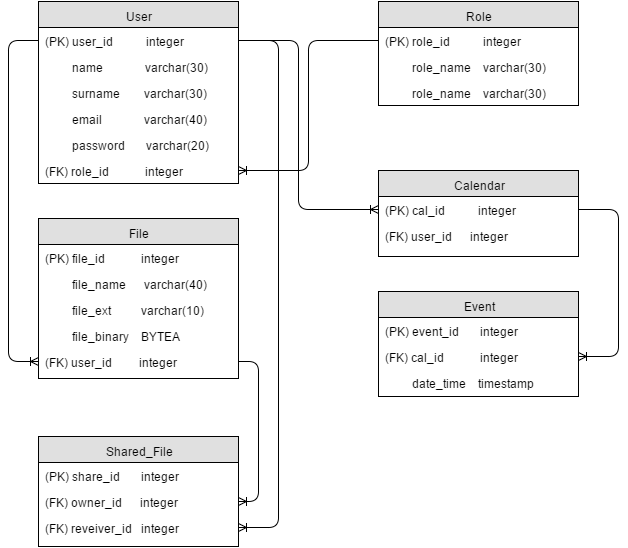
\includegraphics[scale=0.5]{ERD}
\caption{\label{fig:diag_02}Diagram ERD}
\end{figure}

\section{Model klas}
- rowniez jakis ladny wstep \newline
- No i diagram klas tutaj ładnie sklepać trzeba będzie \newline

\section{Diagramy sekwencji}
- Wstep, ze to wynika z diagramu klas, cos ładnego o diagramach sekwencji - tutaj moze sie wykładami szweda posłużyć \newline
- No i wklepac diagramy sekwencji - moze nie bedzie tak zle jak już beda diagramy klas \newline
\section {Projekt interfejsu?}
Nad tym sie zastanowic czy to robic czy dac dupie siana

